\begin{frame}
    \frametitle{Completed Stage I-1: FHR Benchmark Phase I-A Results}
    \begin{itemize}
        \item FHR Benchmark Phase I-A: 2D assembly steady state model
        \item In a recently submitted ANS M$\&$C 2021 conference paper 
        (which I am a co-author on), 
        Petrovic et al. \cite{petrovic_preliminary_2021} compared FHR benchmark 
        participants' Phase I-A $k_{eff}$ results.  
        We reported that the standard deviation between participants for each case 
        was in the 231 to 514 pcm range, acceptable and notably close given a blind 
        benchmark, assuring that \gls{UIUC}'s Phase I-A results are acceptable and 
        in agreement with other benchmark participants 
    \end{itemize}
    \begin{figure}[]
        \begin{minipage}[c]{0.5\textwidth}
        \centering
        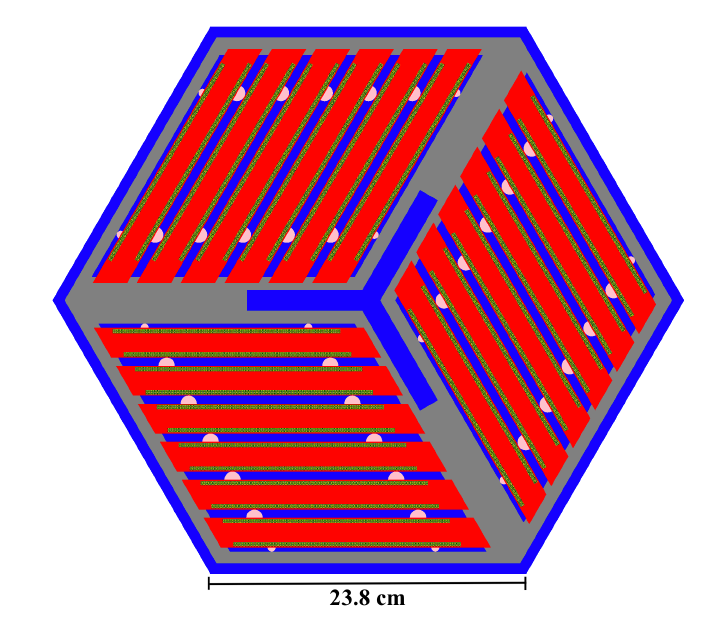
\includegraphics[width=0.75\linewidth]{figures/ahtr-assembly.png} 
        \end{minipage}\hfill
        \begin{minipage}[c]{0.5\textwidth}
        \caption{\acrfull{AHTR} fuel assembly with 18 fuel plates arranged in 
        three diamond-shaped sectors, with a central Y-shaped and external channel 
        graphite structure.}
        \end{minipage}
    \end{figure}
\end{frame}

\begin{frame}
    \frametitle{Completed Stage I-1: FHR Benchmark Phase I-A Results}
    \begin{table}
        \caption{\acrlong{UIUC}'s \acrlong{FHR} Benchmark Phase I-A results 
        \cite{chee_arfcfhr-benchmark_2021}.}
        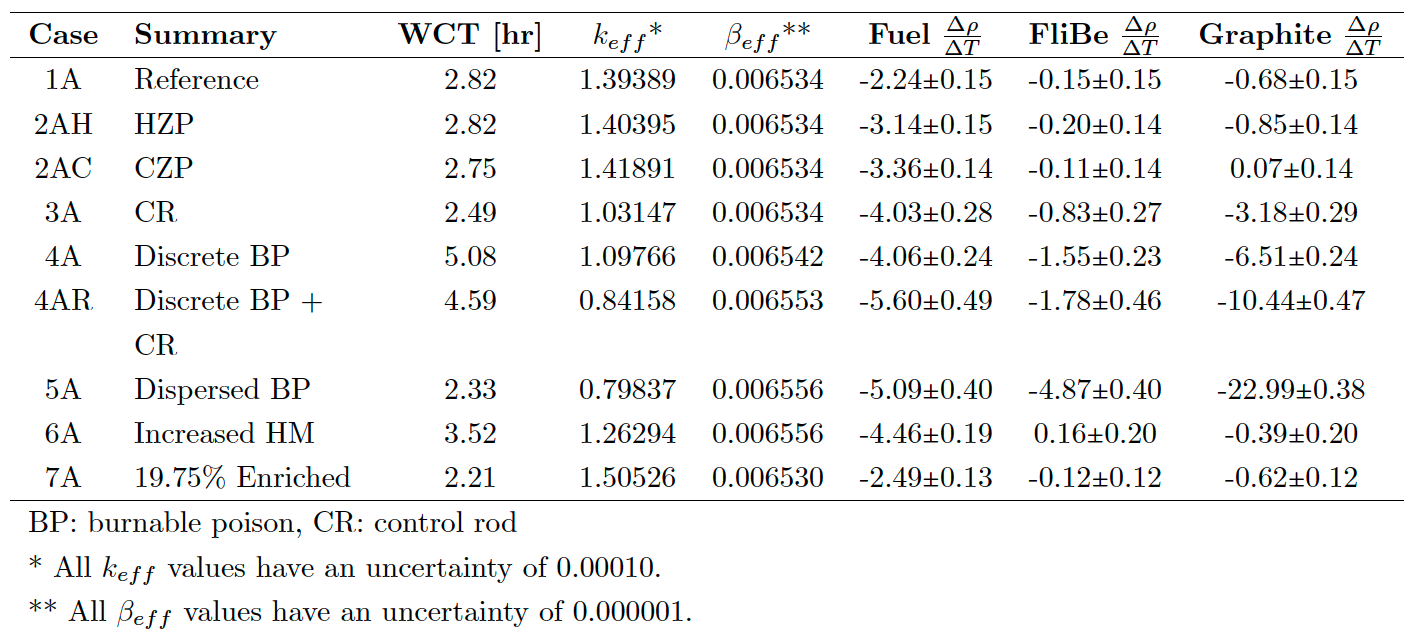
\includegraphics[width=\linewidth]{figures/benchmark-coeff-results.png} 
    \end{table}
\end{frame}

\begin{frame}
    \frametitle{Completed Stage I-1: FHR Benchmark Phase I-A Results}
    \begin{figure}[]
        \centering
        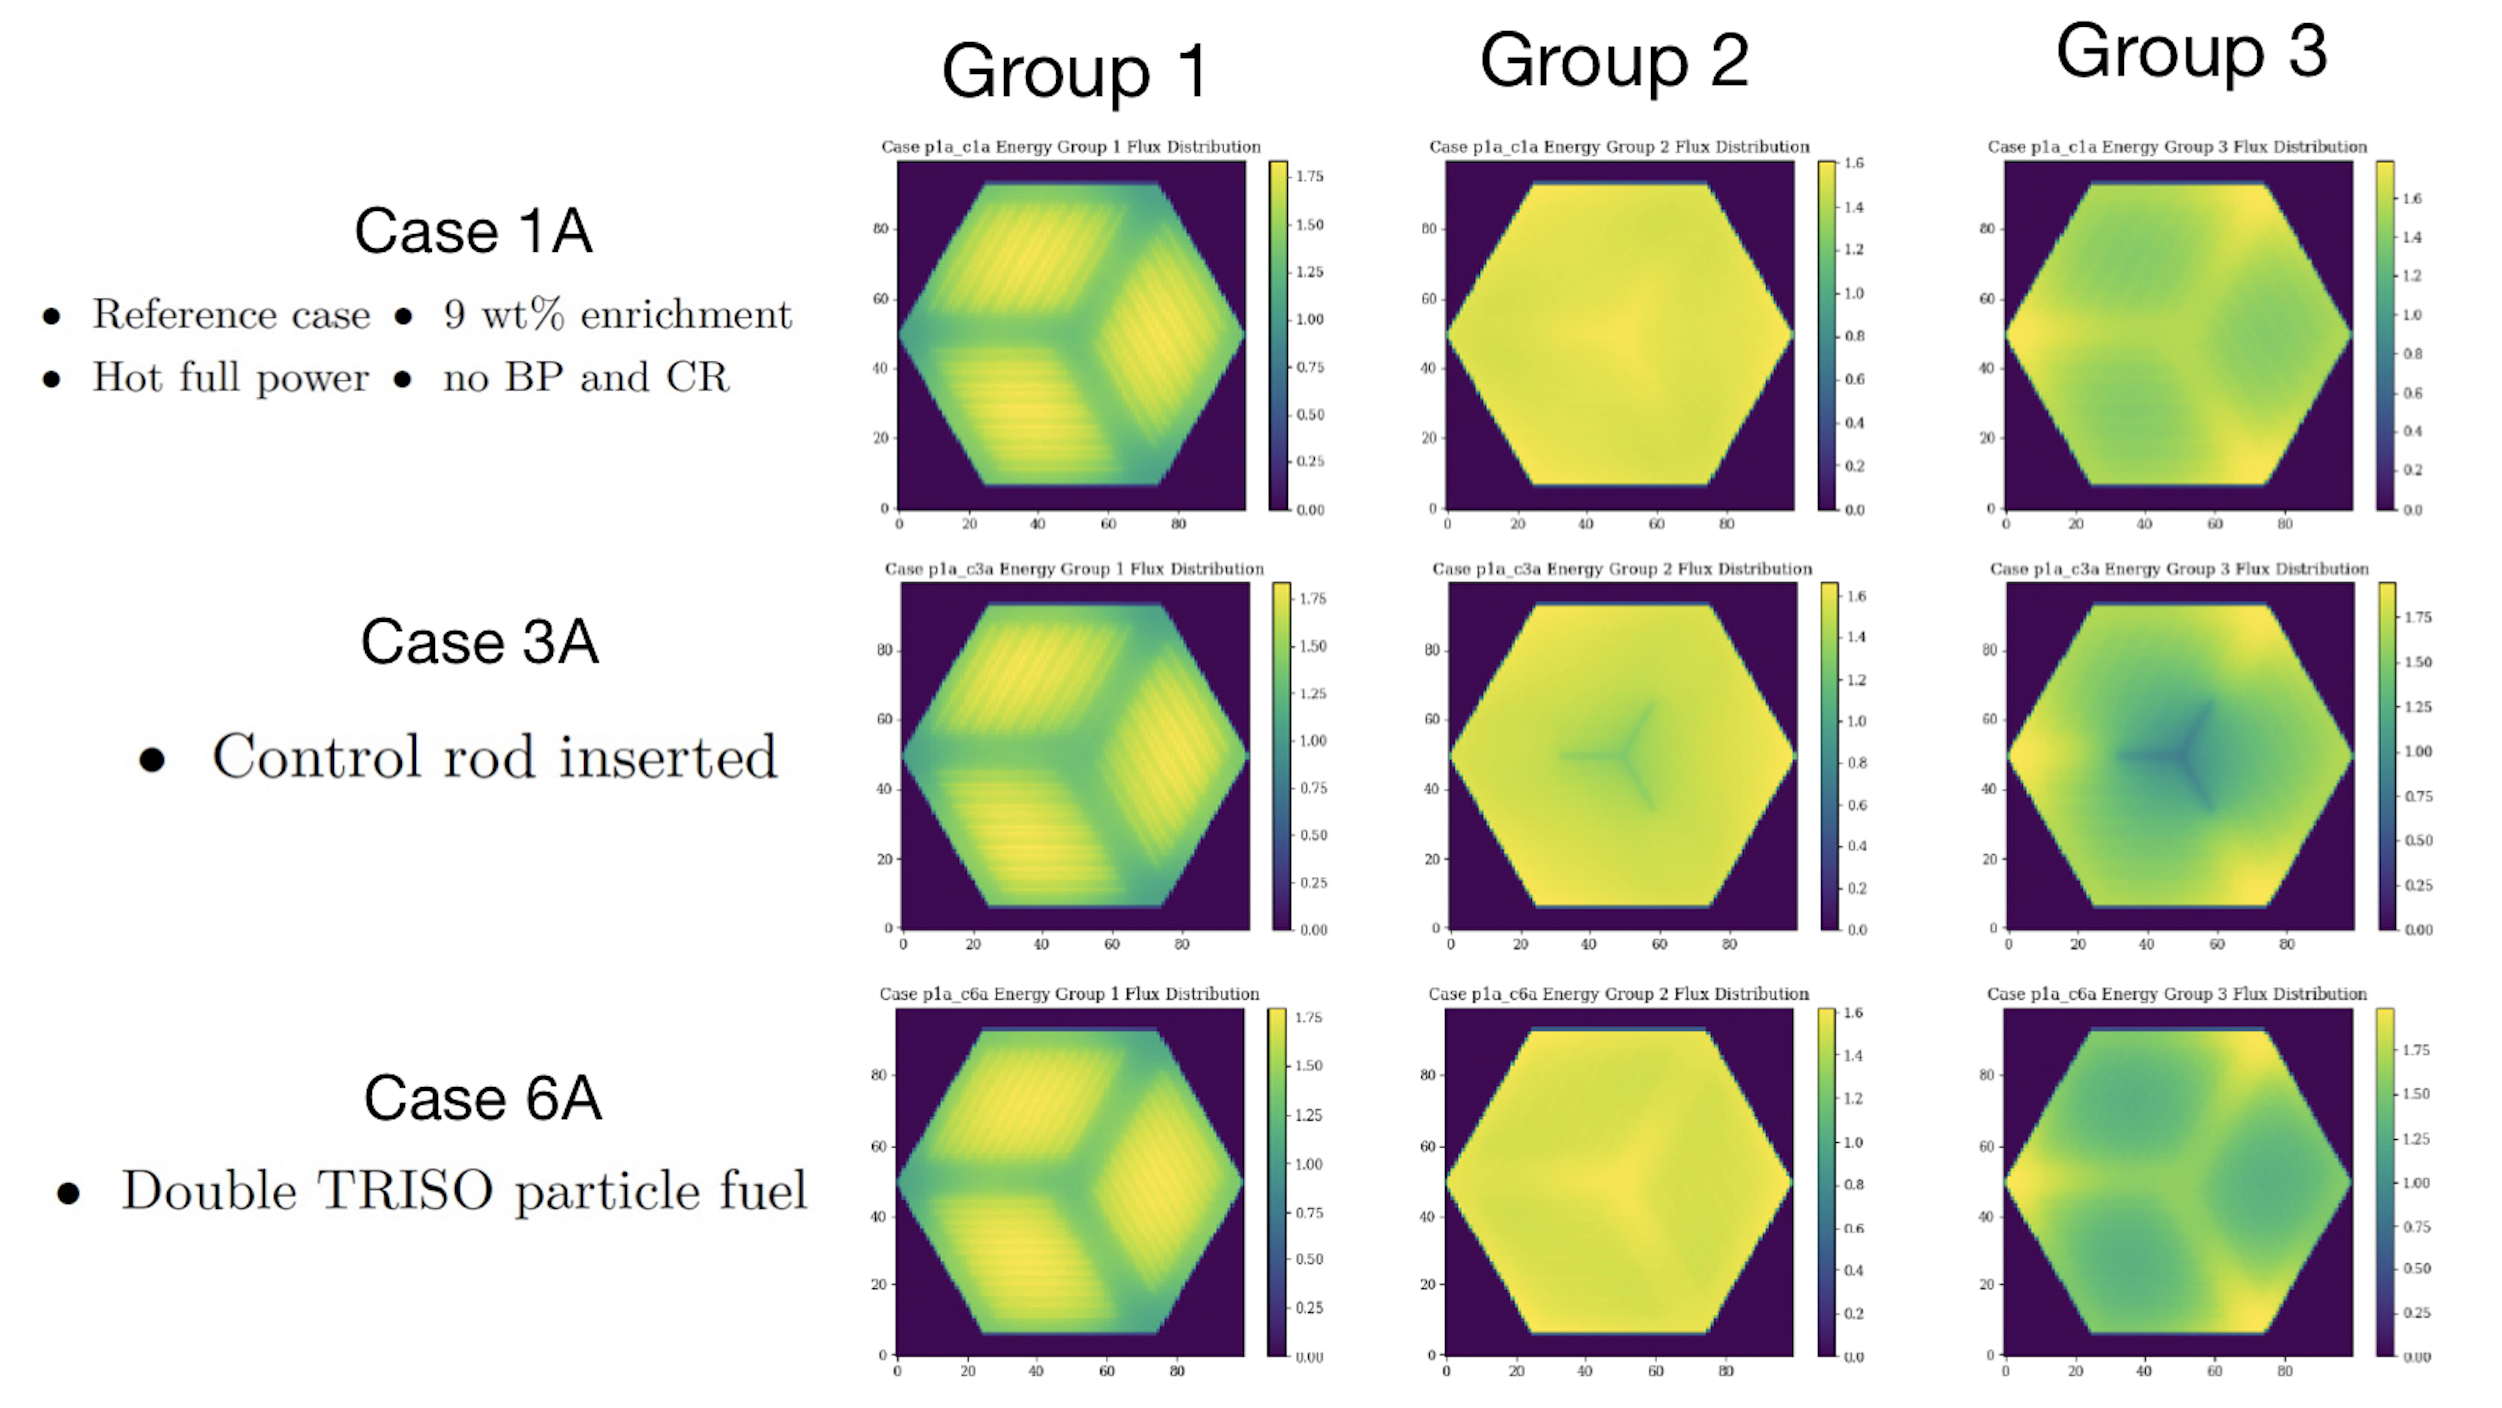
\includegraphics[width=0.6\linewidth]{figures/phase1a-e.png} 
        \caption{UIUC results: FHR Benchmark neutron flux 
        distribution in 100 $\times$ 100 mesh for three coarse energy groups: Case 
        1A (above), Case 3A (middle), Case 6A (below). Energy group 1: $E > 0.1$ MeV, 
        Energy group 2: $3 \times 10^{-6} < E < 0.1$ MeV, Energy group 3: $E < 3 \times 10^{-6}$ MeV. }
    \end{figure}
\end{frame}